\chapter{Notas sobre R}

Aquí escribo algunas notas sobre las funciones y objetos de
\texttt{R} que creo son útiles tener en cuenta.

\section{Sobre los histogramas}
Si \texttt{X} es un vector de números, puedes
usar la función \texttt{hist} para crear un histograma
a partir de los datos numéricos almacenados en 
\texttt{X}.
Pon por ejemplo
\[
\texttt{X} = c(1,1,1,1,2,3). 
\]

\begin{figure}[H]
	\sidecaption{
	Se grafican los histogramas que resultaron 
	de ejecutar, respectivamente, las instrucciones
	\texttt{hist(ame, main = 'freq set as TRUE')}
	y \texttt{hist(ame, main = 'freq set as FALSE', freq = FALSE)}.
	\label{fig: hist 1}
	}
	\centering
	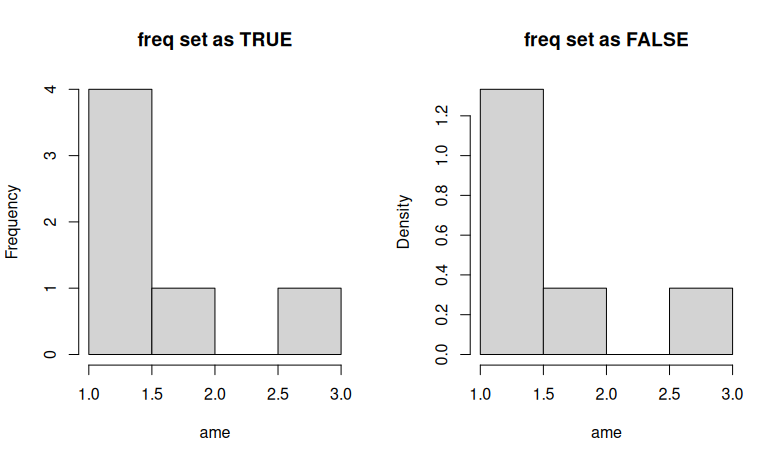
\includegraphics[scale = 0.5]{hist_1} 
\end{figure}	

Como se explica en \cite{hist}, 
poniendo \texttt{freq = FALSE} no da lugar a un histograma
de los \textit{porcentajes} de los valores almacenados en los
datos graficados, sino que normaliza el histograma 
(obviamente respetando proporciones) de tal
forma que el área total de los rectángulos graficados sea $1$. \\

Usar \texttt{freq = FALSE}
parece ser la opción preferida por los autores para graficar
histogramas. No me parece mal, pues se preservan las proporciones
de las ocurrencias, pero personalmente prefiero graficar
las probabilidades de ocurrencia de los elementos de 
\texttt{X}. Para hacer esto, tienes que hacer 
guardar el histograma en una variable (pidiendo no graficarlo)
y modificar la propiedad \texttt{density} de este.

\begin{verbatim}
> h = hist(x, plot = FALSE) 
> h\$density = h\$counts/sum(h\$counts) 
> plot(h,freq=FALSE) 
\end{verbatim}

\begin{figure}[H]
	\sidecaption{
	Histograma que resulta de hacer el cambio
	sugerido en el código de arriba.
	\label{fig: hist 2}
	}
	\centering
	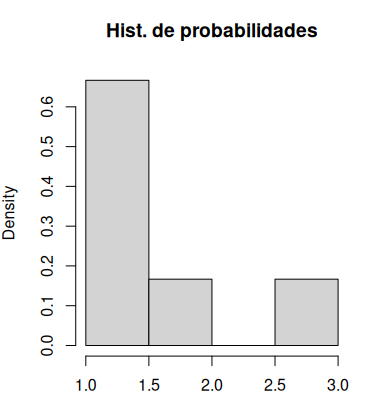
\includegraphics[scale = 0.5]{hist_2} 
\end{figure}	